\chapter{Calculus}

\nomenclature[S_CartSp]{$\mathrm{CartSp}$}{the category of Euclidean spaces and ``suitable'' morphisms (e.g.~linear maps, smooth maps, ...)}

\section{General definitions}

    \newdef{Domain}{\index{domain}
        A connected, open subset of $\mathbb{R}^n$. (Not to be confused with the domain of a function (\cref{set:domain}).)
    }

    \newdef{Factorial}{\index{factorial}\label{calculus:factorial}
        \begin{gather}
            n! := n(n-1)\cdots1\,,
        \end{gather}
        where $n\in\mathbb{N}$. The convention is that $0!=1$. (This for example agrees with the combinatorial result that there is only one way to order zero objects.)
    }

    \newdef{Envelope}{\index{envelope}
        Consider a set $\mathcal{F}$ of real-valued functions with common domain $X$. An envelope (function) for $\mathcal{F}$ is any function $F:X\rightarrow\mathbb{R}$ such that
        \begin{gather}
            \forall f\in\mathcal{F},x\in X:|f(x)|\leq F(x)\,.
        \end{gather}
    }

\section{Sequences}\index{sequence}

    \newdef{Limit superior}{\index{limit}\label{calculus:limit_superior}
        Let $\seq{x}$ be a sequence of real numbers. The limit superior is defined as follows:
        \begin{gather}
            \limsup_{n\rightarrow\infty}x_n := \inf_{n\geq1}\sup_{k\geq n}x_k\,.
        \end{gather}
    }
    \newdef{Limit inferior}{\label{calculus:limit_inferior}
        Let $\seq{x}$ be a sequence of real numbers. The limit superior is defined as follows:
        \begin{gather}
            \liminf_{n\rightarrow\infty}x_n := \sup_{n\geq1}\inf_{k\geq n}x_k\,.
        \end{gather}
    }

    \begin{property}
        A sequence $\seq{x}$ converges pointwise if and only if
        \begin{gather}
            \limsup_{n\rightarrow\infty}x_n = \liminf_{n\rightarrow\infty}x_n\,.
        \end{gather}
    \end{property}

\section{Continuity}\index{continuity}

    \begin{definition}[Darboux function]\index{Darboux!function}
        A function that has the intermediate value property (\cref{topology:intermediate_value_theorem}).
    \end{definition}
    \begin{theorem}[Darboux]\index{Darboux!theorem for differentiable functions}
        Every differentiable function defined on a closed interval has the intermediate value property.
    \end{theorem}
    \begin{result}[Bolzano]\index{Bolzano}
        If $f(a)<0$ and $f(b)>0$ (or vice versa), there exists at least one point $x_0$ for which $f(x_0)=0$.
    \end{result}

    \begin{theorem}[Weierstrass's extreme value theorem]\index{Weierstrass!extreme value theorem}
        Let $I=[a,b]$ be a closed interval and let $f:I\rightarrow\mathbb{R}$ be a continuous function. Then $f$ attains a minimum and maximum at least once on $I$.
    \end{theorem}

    \newdef{Absolute continuity}{\index{continuity!absolute}\label{calculus:absolute_continuity}
        A function $f:\mathbb{R}\rightarrow\mathbb{R}$ is said to be absolutely continuous if for every $\varepsilon>0$ there exists a $\delta_\varepsilon>0$ such that for every finite collection of disjoint intervals $]x_i,y_i[$ satisfying
        \begin{gather}
            \sum_i(y_i-x_i)<\delta_\varepsilon\,,
        \end{gather}
        the function $f$ satisfies
        \begin{gather}
            \sum_i|f(y_i)-f(x_i)|<\varepsilon\,.
        \end{gather}
    }

    \begin{property}
        The different types of continuity form the following hierarchy: \[\text{Lipschitz-continuous}\subset\text{absolutely  continuous}\subset\text{uniformly continuous}\subset\text{continuous}\,.\]
    \end{property}

    \newdef{Function of bounded variation}{\index{bounded!variation}
        A function $f$ is said to be of bounded variation on the interval $[a,b]$ if the following quantity is finite:
        \begin{gather}
            V_{a,b}(f) := \sup_{P\in\mathcal{P}}\sum_{i=0}^{|P|-1}|f(x_{i+1})-f(x_i)|\,,
        \end{gather}
        where the supremum is taken over all partitions of $[a,b]$.
    }
    \begin{property}\label{calculus:bounded_variation_decomposition}
        Every function of bounded variation can be decomposed as the difference of two monotonically increasing functions.
    \end{property}

    \begin{example}
        Every absolutely continuous function is of bounded variation.
    \end{example}

\section{Convergence}\index{convergence}

    \newdef{Pointwise convergence}{
        Let $\seq{f}$ be a sequence of functions. The sequence is said to converge pointwise to a limit function $f$ if
        \begin{gather}
            \forall x\in\dom(f_n):\lim_{n\rightarrow\infty}f_n(x) = f(x)\,.
        \end{gather}
    }
    \newdef{Uniform convergence}{
        Let $\seq{f}$ be a sequence of functions. The sequence is said to converge uniformly to a limit function $f$ if
        \begin{gather}
            \lim_{n\rightarrow\infty}\sup_{x\in\dom(f_n)}|f_n(x) - f(x)| = 0\,.
        \end{gather}
    }

\section{Series}
\subsection{Convergence tests}\index{convergence}

    \begin{property}
        A necessary condition for the convergence of a series $\sum_{i=1}^{+\infty}a_i$ is that
        \begin{gather}
            \lim_{n\rightarrow\infty}a_n=0\,.
        \end{gather}
    \end{property}

    \newprop{Absolute/conditional convergence}{
        If $S'=\sum_{i=1}^{+\infty}|a_i|$ converges, so does $S=\sum_{i=1}^{+\infty}a_i$. In this case, $S$ is said to be absolutely convergent. If $S$ converges but $S'$ does not, $S$ is said to be conditionally convergent.
    }

    \newdef{Majorizing series}{\index{majorization}
        Let $S_a=\sum_{i=1}^{+\infty}a_i$ and $S_b=\sum_{i=1}^{+\infty}b_i$ be two series. The series $S_a$ is said to majorize $S_b$ if for every $k>0$ the partial sums satisfy $S_{a,k}\geq S_{b,k}$, i.e.
        \begin{gather}
            \sum_{i=1}^ka_i\geq\sum_{i=1}^kb_i
        \end{gather}
        for all $k\in\mathbb{N}$.
    }
    \begin{method}[Comparison test]\index{convergence!comparison test}
        Let $S_a,S_b$ be two series such that $S_a$ majorizes $S_b$.
        \begin{itemize}
            \item If $S_b$ diverges, then $S_a$ diverges.
            \item If $S_a$ converges, then $S_b$ converges.
            \item If $S_b$ converges, nothing can be said about $S_a$.
            \item If $S_a$ diverges, nothing can be said about $S_b$.
        \end{itemize}
    \end{method}

    \begin{method}[Maclaurin--Cauchy integral test]\index{convergence!integral test}\index{Maclaurin--Cauchy integral test|see{convergence}}
        Let $f$ be a nonnegative, continuous and monotonically decreasing function defined on the interval $[n,+\infty[$ for some $n\in\mathbb{N}$. If $\int_n^{+\infty}f(x)\,dx$ is convergent, so is $\sum_{k=n}^{+\infty}f(k)$. On the other hand, if the integral is divergent, so is the series.
    \end{method}
    \begin{remark}
        The function does not have to be nonnegative and decreasing on the complete interval. As long as it does on the interval $[N,+\infty[$ for some $N\geq n$, the statement holds. This can be seen by writing $\sum_{k=n}^{+\infty}f(k) = \sum_{k=n}^Nf(k) + \sum_{k=N}^{+\infty}f(k)$ and noting that the first term is always finite (and similarly for the integral).
    \end{remark}

    \begin{property}
        If the integral in the previous theorem converges, the series is bounded in the following way:
        \begin{gather}
            \Int_n^{+\infty} f(x)\,ndx\leq\sum_{i=n}^{+\infty} a_i \leq f(n) + \Int_n^{+\infty} f(x)\,dx\,.
        \end{gather}
    \end{property}

    \begin{method}[d'Alembert's ratio test]\index{convergence!ratio test}\index{d'Alembert!ratio test|see{convergence}}
        Consider the quantity
        \begin{gather}
            R := \lim_{n\rightarrow\infty}\left|\frac{a_{n+1}}{a_n}\right|\,.
        \end{gather}
        The following cases can be distinguished:
        \begin{itemize}
            \item $R<1$: the series converges absolutely.
            \item $R>1$: the series does not converge.
            \item $R=1$: the test is inconclusive.
        \end{itemize}
    \end{method}

    \begin{method}[Cauchy's root test]\index{convergence!root test}\index{Cauchy!root test|see{convergence}}
        Consider the quantity
        \begin{gather}
            R := \limsup_{n\rightarrow\infty}\sqrt[n]{|a_n|}\,.
        \end{gather}
        The following cases can be distinguished:
        \begin{itemize}
            \item $R<1$: the series converges absolutely.
            \item $R>1$: the series does not converge.
            \item $R=1$ and the limit approaches strictly from above: the series diverges.
            \item $R=1$: the test is inconclusive.
        \end{itemize}
    \end{method}
    \newdef{Radius of convergences}{\index{convergence!radius}
        The number $1/R$ is called the radius of convergence.
    }
    \begin{remark}
        The root test is stronger than the ratio test. However, if the ratio test can determine the convergence of a series, the radius of convergence of both tests will coincide and, hence, it is a well-defined quantity.
    \end{remark}

    \begin{method}[Gauss's test]\index{convergence!Gauss's test}\label{series:gauss_test}
        If $a_n>0$ for all $n\in\mathbb{N}$, one can write the ratio of successive terms as follows:
        \begin{gather}
            \left|\frac{a_n}{a_{n+1}}\right| = 1 + \frac{h}{n} + \frac{B(n)}{n^k}\,,
        \end{gather}
        where $k>1$ and $B(n)$ is a bounded function when $n\longrightarrow\infty$. The series converges if $h>1$ and diverges otherwise.
    \end{method}

    \newdef{Asymptotic expansion}{\index{asymptotic!expansion}\label{calculus:asymptotic_expansion}
        Let $f:\mathbb{R}\rightarrow\mathbb{R}$ be a continuous function. A series $\sum_{i=0}^{+\infty}a_nx^n$ is called an asymptotic expansion of $f$ if there exists an $n\in\mathbb{N}$ such that
        \begin{gather}
            f(x) - \sum_{i=0}^na_ix^i = O(x^{n+1})
        \end{gather}
        for all $x\in\mathbb{R}$.
    }

\section{Differentiation}\index{differentiation}

    \newformula{Derivative}{\label{calculus:derivative}
        Consider a function $f:\mathbb{R}\rightarrow\mathbb{R}$. If it exists, the following limit is called the derivative of $f$ at $x\in\mathbb{R}$:
        \begin{gather}
            \deriv{f}{x}\equiv f'(x) := \lim_{h\rightarrow0}\frac{f(x+h)-f(x)}{h}\,.
        \end{gather}
        If the derivative exists at every point of some interval $I$, then $f$ is said to be differentiable on $I$.
        For multivariate functions $f:\mathbb{R}^n\rightarrow\mathbb{R}$ one can similarly define the partial derivatives:
        \begin{gather}
            \pderiv{f}{x_i} := \frac{f(x+he_i)-f(x)}{h}\,,
        \end{gather}
        where $e_i$ is the $i^{th}$ coordinate vector, i.e.~the partial derivatives determine the rate of change in the coordinate directions.
    }

    \begin{theorem}[Mean value theorem]\index{mean!value theorem}\label{calculus:mean_value_theorem}
        Let $f$ be a continuous function defined on the closed interval $[a,b]$ and differentiable on the open interval $]a,b[$. There exists a point $c\in\ ]a,b[$ such that
        \begin{gather}
            f'(c) = \frac{f(b)-f(a)}{b-a}\,.
        \end{gather}
    \end{theorem}

    \newdef{Differentiablity class}{\label{calculus:differentiablity_class}
        A function $f:\mathbb{R}\rightarrow\mathbb{R}$ is said to be of class $C^n$ if it is $n$ times continuously differentiable, i.e.~$f^{(i)}$ exists and is continuous for $i=1,\ldots,n$. Multivariate functions are said to be of class $C^n$ if all of their partial derivatives are.
    }
    \newdef{Smooth function}{\index{smooth!function}\label{calculus:smooth}
        A function $f$ is said to be smooth if it is of class $C^\infty$.
    }

    \begin{theorem}[Boman]\index{Boman}
        Consider a function $f:\mathbb{R}^d\rightarrow\mathbb{R}$. If for every smooth function $g:\mathbb{R}\rightarrow\mathbb{R}^d$ the composition $f\circ g$ is smooth, the function $f$ is also smooth.
    \end{theorem}

    \begin{property}[Taylor expansion]\index{Taylor!expansion}\index{Maclaurin expansion|see{Taylor}}
        Let $f:\mathbb{R}\rightarrow\mathbb{R}$ be a smooth function. Around every point $x\in\mathbb{R}$, one can express $f$ as the following series:
        \begin{gather}
            f(y) = f(x) + f'(x)(y-x) + \frac{f''(x)}{2}(y-x)^2 + \cdots = \sum_{n=0}^{+\infty}\frac{f^{(n)}(x)}{n!}(y-x)^n\,.
        \end{gather}
        For the special case $x=0$ the name \textbf{Maclaurin series} is sometimes used. A similar expression exists for multivariate functions, where derivatives are replaced by partial derivatives.
    \end{property}

    \newdef{Analytic function}{\index{analytic!function}\label{calculus:analytic}
        \nomenclature[S_Comega]{$C^\omega(V)$}{the set of all analytic functions defined on the set $V$}
        A function $f$ is said to be analytic if it is smooth and if its Taylor series expansion around any point $x$ converges to $f$ in some neighbourhood of $x$. The set of analytic functions defined on $V$ is denoted by $C^\omega(V)$.
    }

    \begin{theorem}[Hadamard lemma]\index{Hadamard!lemma}
        Let $f:\mathbb{R}^n\rightarrow\mathbb{R}$ be a smooth function defined on an open, star-convex set $U$. One can expand the function as follows:
        \begin{gather}
            f(x) = f(x_0) + \sum_{i=1}^n(x^i-x^i_0)g_i(x_0)\,,
        \end{gather}
        where all functions $g_i$ are also smooth on $U$.
    \end{theorem}
    From this expression one can also see that the functions $g_i$, evaluated at 0, give the partial derivatives of $f$. These functions are sometimes called the \textbf{Hadamard quotients}.
    \remark{This lemma gives a finite order approximation of the Taylor expansion of $f$.}

    \begin{theorem}[Schwarz\footnotemark]\index{Schwarz}\index{Clairaut}\label{calculus:schwarz_theorem}
        \footnotetext{Also called \textbf{Clairaut's theorem}.}
        Consider a twice differentiable function $f\in C^2(\mathbb{R}^n,\mathbb{R})$. The mixed partial derivatives of $f$ coincide for all indices $i,j\leq n$:
        \begin{gather}
            \pderiv{}{x_i}\left(\pderiv{f}{x_j}\right) = \pderiv{}{x_j}\left(\pderiv{f}{x_i}\right)\,.
        \end{gather}
    \end{theorem}

    \begin{formula}[Derivative of \texorpdfstring{$f(x)^{g(x)}$}{f(x)^g(x)}]\label{calculus:derivative_f^g}
        Consider a function of the form \[u(x)=f(x)^{g(x)}\,,\] with $f,g:\mathbb{R}\rightarrow\mathbb{R}$ differentiable. After taking the logarithm and applying the standard rules of differentiation, one can obtain the following expression:
        \begin{gather}
            \left(f(x)^{g(x)}\right)' = f(x)^{g(x)}\left(g'(x)\ln\bigl[f(x)\bigr] + \frac{g(x)}{f(x)}f'(x)\right)\,.
        \end{gather}
    \end{formula}

    \newdef{Euler operator}{\index{Euler!operator}\label{calculus:euler_operator}
        On the space $C^{n>1}(\mathbb{R}^n,\mathbb{R})$, the Euler operator $\mathbb{E}$ is defined as follows:
        \begin{gather}
            \mathbb{E} := \sum_{i=1}^nx_i\pderiv{}{x^i}\,.
        \end{gather}
    }
    \begin{theorem}[Euler]\index{homogeneous!function}\index{Euler!homogeneous function theorem}\label{calculus:euler_homogeneous_functions}
        Let $f$ be a homogeneous function, i.e.
        \begin{gather}
            f(\lambda x_1,\ldots,\lambda x_n) = \lambda^nf(x_1,\ldots,x_n)\,.
        \end{gather}
        This function satisfies the following equality:
        \begin{gather}
            \mathbb{E}(f) = nf(x_1,\ldots,x_n)\,.
        \end{gather}
    \end{theorem}

\section{Integration theory}
\subsection{Riemann integral}\index{integral!Riemann}\index{Riemann|seealso{integral}}

    \newdef{Improper Riemann integral}{\label{calculus:improper_integral}
        \begin{gather}
            \Int_{-\infty}^{+\infty}f(x)\,dx := \lim_{\substack{a\rightarrow-\infty\\b\rightarrow+\infty}}\Int_a^bf(x)\,dx
        \end{gather}
        One-sided improper integrals are defined in a similar fashion.
    }

    \begin{theorem}[First fundamental theorem of calculus]\index{fundamental theorem!of calculus}\label{calculus:first_fundamental_theorem}
        Let $f$ be a continuous function defined on an open interval $I$ and consider any number $c\in I$. The following expression establishes the relation between integration and differentiation:
        \begin{gather}
            \exists F\in C^1(I):\forall x\in I:F'(x)=f(x)\,.
        \end{gather}
        Furthermore, the function $F$ is uniformly continuous on $I$ and is given by the following integral:
        \begin{gather}
            F(x) = \Int_c^xf(x')\,dx'\,.
        \end{gather}
    \end{theorem}

    \begin{remark}
        The function $F$ in the previous theorem is called a \textbf{primitive (function)} of $f$. Remark that $F$ is just `a' primitive function, since adding a constant to $F$ does not change anything because the derivative of a constant is zero (the number $c\in\mathbb{R}$ was arbitrary).
    \end{remark}

    \begin{theorem}[Second fundamental theorem of calculus]\label{calculus:second_fundamental_theorem}
        Let $f$ be a $C^1$-function on the interval $[a,b]$.
        \begin{gather}
            \Int_a^bf'(x)\,dx = f(b) - f(a)
        \end{gather}
    \end{theorem}

    \begin{formula}[Differentiation under the integral sign\footnotemark]\index{Leibniz!integral rule}\label{calculus:leibniz_integral_rule}
        \footnotetext{This is a more general version of the \textit{Leibniz integral rule}.}
        \begin{gather}
            \deriv{}{x}\Int_{a(x)}^{b(x)}f(x,y)\,dy = f\bigl(x,b(x)\bigr)b'(x) - f\bigl(x,a(x)\bigr)a'(x) + \Int_{a(x)}^{b(x)}\pderiv{f(x,y)}{x}\,dy
        \end{gather}
    \end{formula}

    \newdef{Borel transform}{\index{Borel!transform}\label{calculus:borel_transform}
        Consider the following function:
        \begin{gather}
            F(x) := \sum_{n=0}^{+\infty}\frac{a_n}{n!}x^n\,.
        \end{gather}
        If
        \begin{gather}
            \Int_0^{+\infty}e^{-t}F(xt)\,dt<+\infty
        \end{gather}
        for all $x\in\mathbb{R}$, then $F$ is called the Borel transform of
        \begin{gather}
            f(x) = \sum_{n=0}^{+\infty}a_nx^n\,.
        \end{gather}
        Furthermore, the integral gives a convergent expression for $f$.
        \begin{mdframed}[roundcorner=10pt, linecolor=blue, linewidth=1pt]
            \begin{proof}
                The function $F$ is defined as follows:
                \begin{gather}
                    F(x) := \sum_{n=0}^{+\infty}\frac{a_n}{n!}x^n\,.
                \end{gather}
                The Borel transform gives:
                \begin{align*}
                    \Int_0^{+\infty}F(xt)e^{-t}\,dt&=\sum_{n=0}^N\Int_0^{+\infty}\frac{a_n}{n!}x^nt^ne^{-t}\,dt\\
                    &=\sum_{n=0}^N\frac{a_n}{n!}x^n\Int_0^{+\infty}t^ne^{-t}\,dt\\
                    &=\sum_{n=0}^N\frac{a_n}{n!}x^n\,\Gamma(n+1)\\
                    &=\sum_{n=0}^Na_nx^n\,,
               \end{align*}
               where the definition of the Gamma function (\cref{calculus:gamma_function}) was used on line 3, and the relation~\eqref{calculus:gamma_factorial_relation} between the factorial function and the Gamma function was used on line 4.
            \end{proof}
        \end{mdframed}
    }

    \begin{theorem}[Watson]\index{Watson}
        The Borel transform $F$ is unique if the function $f$ is holomorphic (\cref{complexcalculus:holomorphic}) on the domain $\{z\in\mathbb{C}\mid|\arg(z)|<\frac{\pi}{2}+\varepsilon\}$.
    \end{theorem}

\subsection{Euler integrals}\index{Euler!integral}

   \newformula{Beta function}{\index{beta function}\label{calculus:beta_function}
       The beta function (also known as the \textbf{Euler integral of the first kind}) is defined as follows:
        \begin{gather}
            B(x,y) := \Int_0^1t^{x-1}(1-t)^{y-1}\,dt\,.
        \end{gather}
    }

   \newformula{Gamma function}{\index{gamma!function}\label{calculus:gamma_function}
       The gamma function (also known as the \textbf{Euler integral of the second kind}) is defined as follows:
        \begin{gather}
            \Gamma(x) := \Int_0^{+\infty}t^{x-1}e^{-t}\,dt\,.
        \end{gather}
    }

    \begin{formula}
        The following formula relates the beta and gamma functions:
        \begin{gather}
            B(x,y) = \frac{\Gamma(x)\Gamma(y)}{\Gamma(x+y)}\,.
        \end{gather}
    \end{formula}

    \begin{property}[Recursion]
        The gamma function satisfies the following recursion relation for all points $x$ in its domain:
        \begin{gather}
            \Gamma(x+1)=z\Gamma(x)\,.
        \end{gather}
    \end{property}

    \newformula{Factorial}{\label{calculus:gamma_factorial_relation}
        For integers $n\in\mathbb{N}$ the gamma function can be expressed in terms of the factorial (\cref{calculus:factorial}):
        \begin{gather}
            \Gamma(n) = (n-1)!\,.
        \end{gather}
    }
    \newformula{Stirling}{\index{Stirling}\label{calculus:stirling}
        This formula (originally stated for the factorial of natural numbers) gives an asymptotic expansion of the gamma function:
        \begin{gather}
            \ln\Gamma(z) \approx z\ln z - z + \frac{1}{2}\ln\left(\frac{2\pi}{z}\right)\,.
        \end{gather}
    }

\subsection{Gaussian integrals}\index{Gauss!integral}

    \newformula{$n$-dimensional Gaussian integral}{\index{Wick!lemma}
        An integral of the form
        \begin{gather}
            I\left(A,\vector{b}\right) := \Int_{\mathbb{R}^n}\exp\left(-\frac{1}{2}\vector{x}\cdot A\vector{x} + \vector{b}\cdot\vector{x}\right)\,d^nx\,,
        \end{gather}
        where $A$ is a real symmetric matrix. By performing the transformation $\vector{x}\rightarrow A^{-1}\vector{b}-\vector{x}$ and diagonalizing $A$, one can obtain the following expression:
        \begin{gather}
            \label{calculus:gaussian_integral}
            I\left(A,\vector{b}\right) = \sqrt{\frac{(2\pi)^n}{\det(A)}}\exp\left(\frac{1}{2}\vector{b}\cdot A^{-1}\vector{b}\right)\,.
        \end{gather}
        More generally, one has the following result:
        \begin{gather}
            \Int_{\mathbb{R}^n}\exp\left(-\frac{1}{2}\vector{x}\cdot A\vector{x}\right)f(\vector{x})\,d^nx = \sqrt{\frac{(2\pi)^n}{\det(A)}}\left.\exp\left(\frac{1}{2}\sum_{i,j=1}^nA^{-1}_{ij}\partial_i\partial_j\right)f(\vector{x})\right|_{\vector{x}=0}\,.
        \end{gather}
        This result is sometimes called \textbf{Wick's lemma}.
    }
    \begin{result}
        A functional generalization is given by:
        \begin{align}
            I(iA,iJ) &= \Int\exp\left(-i\Int_{\mathbb{R}^n\times\mathbb{R}^n}\varphi(x)A(x,y)\varphi(y)\,d^nx\,d^ny + i\Int_{\mathbb{R}^n}\varphi(x)J(x)\,d^nx\right)[d\varphi]\nonumber\\
            &= C\det(A)^{-1/2}\exp\left(\frac{i}{2}\Int_{\mathbb{R}^n\times\mathbb{R}^n}J(x)A^{-1}(x,y)J(y)\,d^nx\,d^ny\right)\,,
        \end{align}
        where the analytic continuation $I(iA,iJ)$ of \cref{calculus:gaussian_integral} was used. One should pay attention to the normalization factor $C$ which is infinite in general.
    \end{result}

    \begin{method}[Feynman diagrams]\index{Feynman!diagram}
        The expansion of the exponential in the general expression for Gaussian integrals admits a diagrammatic expression. Let $f(\vector{x})$ be a polynomial function of the coordinates.

        If the number of factors in a monomial is odd, the resulting integral will vanish (since the integral of an odd function over an even domain is zero). For an even number of factors one gets the following expression:
        \begin{gather}
            \Int_{\mathbb{R}^n}\exp\left(-\frac{1}{2}\vector{x}\cdot A\vector{x}\right)x^{i_1}\cdots x^{i_k}\,d^nx = \sqrt{\frac{(2\pi)^n}{\det(A)}}\sum_{\sigma\in S_k}A^{-1}_{\sigma(i_1)\sigma(i_2)}\cdots A^{-1}_{\sigma(i_{k-1})\sigma(i_k)}\,.
        \end{gather}
        To every coordinate dimension one can assign a vertex in the place, i.e.~the object $x_i$ can be interpreted as a real-valued function on the set of $k$ elements. The sum on the right-hand side above can then be expressed as a `sum' over all possible diagrams, where a factor $A^{-1}_{ij}$ is represented by a line connecting the vertices $i$ and $j$.
    \end{method}

    \begin{example}[Feynman diagrams]
        Some simple examples are given:
        \begin{gather*}
            A^{-1}_{13}A^{-1}_{12}A^{-1}_{24} =
            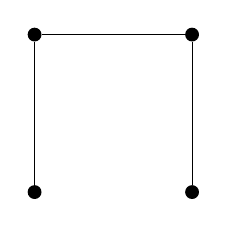
\begin{tikzpicture}[baseline={([yshift=-.5ex]current bounding box.center)}]
                \node[fill, circle, inner sep = 0, minimum size = 5pt] at (0, 0) (1) {};
                \node[fill, circle, inner sep = 0, minimum size = 5pt] at (2, 0) (2) {};
                \node[fill, circle, inner sep = 0, minimum size = 5pt] at (0, -2) (3) {};
                \node[fill, circle, inner sep = 0, minimum size = 5pt] at (2, -2) (4) {};
                \draw (1) -- (2);
                \draw (1) -- (3);
                \draw (2) -- (4);
            \end{tikzpicture}
        \end{gather*}
        Higher powers of a given coordinate would then for example give rise to diagrams with loops at a given vertex:
        \begin{gather*}
            A^{-1}_{11}A^{-1}_{12}A^{-1}_{22} =
            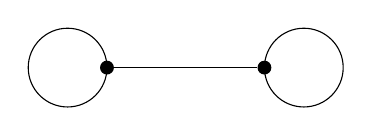
\begin{tikzpicture}[baseline={([yshift=-.5ex]current bounding box.center)}]
                \node[fill, circle, inner sep = 0, minimum size = 5pt] at (0, 0) (1) {};
                \node[fill, circle, inner sep = 0, minimum size = 5pt] at (2, 0) (2) {};
                \draw (-0.5, 0) circle (0.5);
                \draw (1) -- (2);
                \draw (2.5, 0) circle (0.5);
            \end{tikzpicture}
        \end{gather*}
    \end{example}

    \begin{remark}[Normalization]
        In practice one often divides all Gaussian integrals by the quantity $I(A,0)$ to cancel the normalization factor. In the functional setting this even imperative since, as mentioned above, the normalization factor diverges for infinite-dimensional spaces.
    \end{remark}

\subsection{Generalizations}

    \newdef{Henstock--Kurzweil integral\footnotemark}{\index{integral!Henstock--Kurzweil}\index{integral!Perron}\index{integral!Denjoy}\index{integral!Luzin}\index{gauge|seealso{integral}}\index{integral!McShane}
    \footnotetext{Also called the \textbf{Perron}, \textbf{Lusin}, \textbf{(narrow) Denjoy} or \textbf{gauge} integral.}
        Consider the usual definition of the (proper) Riemann integral, where tagged partitions $P$ of $[a,b]$ are chosen and the integral is obtained as the limit of the Riemann sums
        \begin{gather}
            I = \sum_Pf(x_i)(t_i-t_{i-1})
        \end{gather}
        as the mesh size of the partitions goes to zero.

        Now, to obtain the generalized integral, consider a strictly positive function $\delta:[a,b]\mathbb{R}^{>0}$, the \textbf{gauge function}. Given such a gauge, a tagged partition $P$ is said to be \textbf{$\delta$-fine} if
        \begin{gather}
            [t_{i-1},t_i]\subset[x_i-\delta(x_i),x_i+\delta(x_i)]
        \end{gather}
        for subintervals in the partition.\footnote{If the condition $x_i\in[t_{i-1},t_i]$ in the definition of tagged partitions is dropped, the \textbf{McShane integral} is obtained. This can be shown to be equivalent to the \textbf{Lebesgue integral} (see \cref{chapter:measure}).}

        If the integral exists, it is given by the number $I\in\mathbb{R}$ such that for all $\varepsilon>0$ there exists a gauge $\delta:[a,b]\rightarrow\mathbb{R}^{>0}$ such that if $P$ is $\delta$-fine, then
        \begin{gather}
            \left\vert I-\sum_Pf(x_i)(t_i-t_{i-1})\right\vert<\varepsilon\,.
        \end{gather}
    }
    \begin{remark}[Riemann integral]
        If the gauge functions are chosen to be constant, the classical $(\varepsilon,\delta)$-definition of ordinary Riemann integrals is obtained.
    \end{remark}

    The following statement can be seen as a refinement of \cref{topology:heine_borel}. Moreover, it is also sometimes known as the \textbf{Borel--Lebesgue theorem}.\index{Borel--Lebesgue}
    \begin{property}[Cousin]\index{Cousin}
        For every gauge $\delta:[a,b]\rightarrow\mathbb{R}^{>0}$, there exists a $\delta$-fine partition. 
    \end{property}

    \begin{property}[Integrability]
        If $f:[a,b]\rightarrow\mathbb{R}$ is bounded, then the following are equivalent:
        \begin{itemize}
            \item $f$ is Henstock--Kurzweil integrable, and
            \item $f$ is \textit{Lebesgue integrable} (see \cref{chapter:measure}).
        \end{itemize}
        More generally, a function $f:[a,b]\rightarrow\mathbb{R}$ is Henstock--Kurzweil integrable if and only if both $f$ and $|f|$ are \textit{Lebesgue integrable}.
    \end{property}

    The following property shows that `improper' Henstock--Kurzweil integrals are only truly improper for unbounded domains.
    \begin{property}[Hake]\index{Hake}
        \begin{gather}
            \Int_a^bf\,dx = \lim_{c\nearrow b}\Int_a^cf\,dx\,,
        \end{gather}
        whenever either side exists.
    \end{property}

\section{Convexity}

    \newdef{Convex set}{\index{convex}\index{hull}\label{calculus:convex}
        A subset of $X$ of a vector space $V$ (\cref{linalgebra:vector_space}) is said to be convex if $x,y\in X$ implies that $\bigl\{\lambda x+(1-\lambda)y\mid\lambda\in[0,1]\bigr\}\subset X$, i.e.~if all straight lines connecting elements of the set are completely contained in that set. The \textbf{convex hull} of a subset $X$ is defined as the smallest convex subset containing $X$.
    }

    \newdef{Convex function}{
        Let $X$ be a convex set. A function $f:X\rightarrow\mathbb{R}$ is said to be convex if for all $x,y\in X$ and $\lambda\in[0,1]$:
        \begin{gather}
            f\bigl(\lambda x + (1-\lambda)y\bigr)\leq t\lambda(x) + (1-\lambda)f(y)\,.
        \end{gather}
        For the definition of a \textbf{concave} function, the inequality has to be turned around.
    }
    \begin{definition}[Linear map]\index{linear!map}
        A function $f:X\rightarrow\mathbb{R}$ is linear if and only if it is both convex and concave.
    \end{definition}

    \begin{theorem}[Karamata's inequality]\index{Karamata}
        Consider an interval $I\subset\mathbb{R}$ and let $f:I\rightarrow\mathbb{R}$ be a convex function. If $(x_1,\ldots,x_n)$ is a tuple that majorizes $(y_1,\ldots,y_n)$, i.e.
        \begin{gather}
            \sum_{i=1}^nx_i = \sum_{i=1}^ny_i
        \end{gather}
        and
        \begin{gather}
            x_{(1)} + \cdots + x_{(k)}\geq y_{(1)} + \cdots + y_{(k)}
        \end{gather}
        for all $k\leq n$, where $x_{(i)}$ denotes the $i^{th}$ largest element of $(x_1,\ldots,x_n)$, then
        \begin{gather}
            \sum_{i=1}^nf(x_i)\geq\sum_{i=1}^nf(y_i)\,.
        \end{gather}
    \end{theorem}

    The following inequality can be derived directly from the definition of convexity by induction.
    \begin{theorem}[Jensen's inequality]\index{Jensen's inequality}\label{calculus:jensen_inequality}
        Let $f$ be a convex function and consider a point $\{a_i\}_{i\leq n}$ in the probability simplex $\Delta^n$ (\cref{topology:standard_simplex}).
        \begin{gather}
            f\left(\sum_{i=1}^na_ix_i\right)\leq\sum_{i=1}^na_if(x_i)\,.
        \end{gather}
    \end{theorem}

    \newdef{Legendre transformation}{\index{Legendre!transformation}\label{calculus:legendre}
        Consider a function $f:\mathbb{R}\rightarrow\mathbb{R}$. In certain cases (especially in physics) it is sometimes useful to replace the argument $x$ by the slope of $f$ at $x$, i.e.~to perform the transformation
        \begin{gather}
            x\longrightarrow f'(x)\,.
        \end{gather}
        However, it should be clear that this transformation is not always well-defined and, even if it is, it does not always preserve all the information contained in $f$.

        These conditions are satisfied exactly if $f$ is convex (or concave). In this case, the Legendre transform of $f$ is defined as
        \begin{gather}
            f^*(x^*) := \sup_x\bigl(x^*x - f(x)\bigr)\,.
        \end{gather}
        Now, consider the case where $f$ is differentiable. The above supremum can then be obtained by differentiating the right-hand side and equating it to zero. This results in $x^* = f'(x)$, which is exactly the transformation that was required. By expressing everything in terms of the Legendre tranformed quantity $x^*$, one can also find the derivative of $f^*$:
        \begin{gather}
            \deriv{f^*}{x^*}(x^*) = x(x^*)\,.
        \end{gather}
    }

    \begin{property}[Alternative characterization]\label{calculus:legendre_condition}
        In fact, up to an additive constant, the condition
        \begin{gather}
            (f^*)' = (f')^{-1}
        \end{gather}
        uniquely determines the Legendre transformation.
    \end{property}
    \begin{remark}
        The above definitions can easily be extended to higher dimensions ($n\geq2$).
    \end{remark}